% TeX encoding = utf8
% TeX spellcheck = pl_PL 
\documentclass[a4paper, 12pt]{article}
\usepackage[utf8]{inputenc}
\usepackage[polish]{babel}
\usepackage{polski}
\usepackage{graphicx}
\usepackage{listings}
\usepackage{amsfonts}
\usepackage{geometry}
\usepackage{indentfirst}
\usepackage{subfigure}
\usepackage{url}
\usepackage{listings}
\usepackage{color}
\usepackage[usenames,dvipsnames]{xcolor}

%\renewcommand*{\addcontentsline}[3]{\addtocontents{#1}{\protect\contentsline{#2}{#3}{}}}
\newgeometry{tmargin=2.5cm, bmargin=2.5cm, lmargin=3.5cm, rmargin=2.5cm}
%\setcounter{secnumdepth}{2}
\setlength{\fboxsep}{0pt}
\lstset{
	basicstyle=\footnotesize\ttfamily,
	breaklines=true,
	language=Python,
	breakatwhitespace=true,
	frame=leftline,
	numbers=left,
	numberstyle=\tiny,
	commentstyle=\color{Gray}\footnotesize\ttfamily}


\author{Anna Wujek \\ Łukasz Korpal \\ Wiktor Ślęczka}
\title{Analiza zagadnienia i przygotowanie środowiska roboczego \\ {\large Roboty monitorujace skażenie środowiska - symulator V-REP}}

\begin{document}
	\sloppy
	\maketitle
	\section{Zadanie}
	Celem projektu jest projekt oraz implementacja symulatora mobilnej sieci ad hoc (MANET) do monitorowania skażenia środowiska naturalnego. Węzłami sieci będą roboty mobilne, wyposażone w czujniki oraz komunikujące się między sobą. Zadaniem robotów będzie lokalizacja chmury skażenia i otoczenie jej robotami, monitorującymi jej położenie i granice, przy założeniu utrzymania spójności sieci.
	
	\subsection{Założenia}
	\begin{itemize}
		\item Roboty potrafią się na bieżąco lokalizować.
		\item System składa się z pewnej liczby robotów mobilnych oraz jednostki centralnej odbierającej od robotów dane o skażeniu.
		\item Roboty mobilne działają autonomicznie i potrafią same zorganizować sieć.
		\item Roboty są wyposażone w czujniki pozwalające im wykrywać poziom skażenia oraz przeszkody.
		\item Roboty są wyposażone w urządzenia pozwalające im się między sobą komunikować, z pewnymi ograniczeniami.
		\item Chmura skażenia jest spójna, może się przemieszczać i zmieniać kształt.
	\end{itemize}
	
	\subsection{Scenariusz działania}
		
		Nieznana jest mapa przestrzeni roboczej oraz lokalizacja chmury skażenia. Roboty są autonomiczne w zakresie omijania przeszkód, a także same organizują się w sieć, a do jednostki centralnej tylko wysyłają dane o skażeniu. Ważne jest w tym przypadku dbanie o zachowanie spójności sieci, zwłaszcza podczas omijania przeszkód. Chmura może się przemieszczać oraz zmieniać kształt w trakcie zadania. Roboty poszukują granic chmury oraz starają się ją całkowicie otoczyć.
		
		
	
	\subsection{Narzędzia}
	Wykorzystany zostanie symulator V-rep w połączeniu z językiem skryptowym python. V-rep posłuży jako symulator przestrzeni roboczej oraz robotów i ich czujników, natomiast w języku Python zaimplementowana zostanie jednostka centralna oraz logika robotów.
	
	W ramach przygotowania środowiska stworzyliśmy niewielki program do sterowania robotem z zewnętrznego skryptu, który uruchamia silnik robota i odczytuje stan czujników. 
	
	\begin{figure}[h!]
	\centering
	\frame{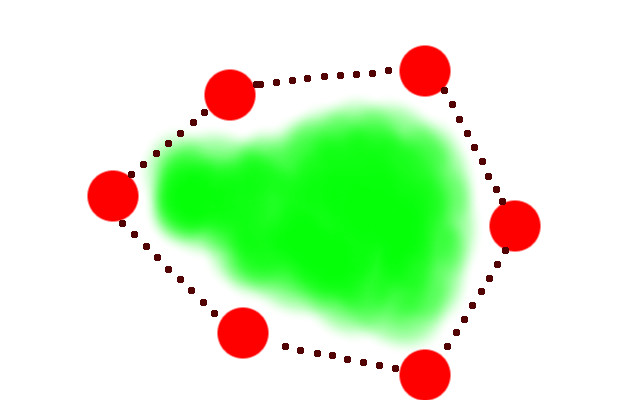
\includegraphics[width=0.7\columnwidth]{img/chmura.jpg}}
	\caption{Przykładowy sposób otoczenia chmury skażenia przez roboty.}
	\end{figure}
		
	\clearpage
	\subsection{Wstępny projekt systemu}	
	\begin{figure}[h!]
	\centering
	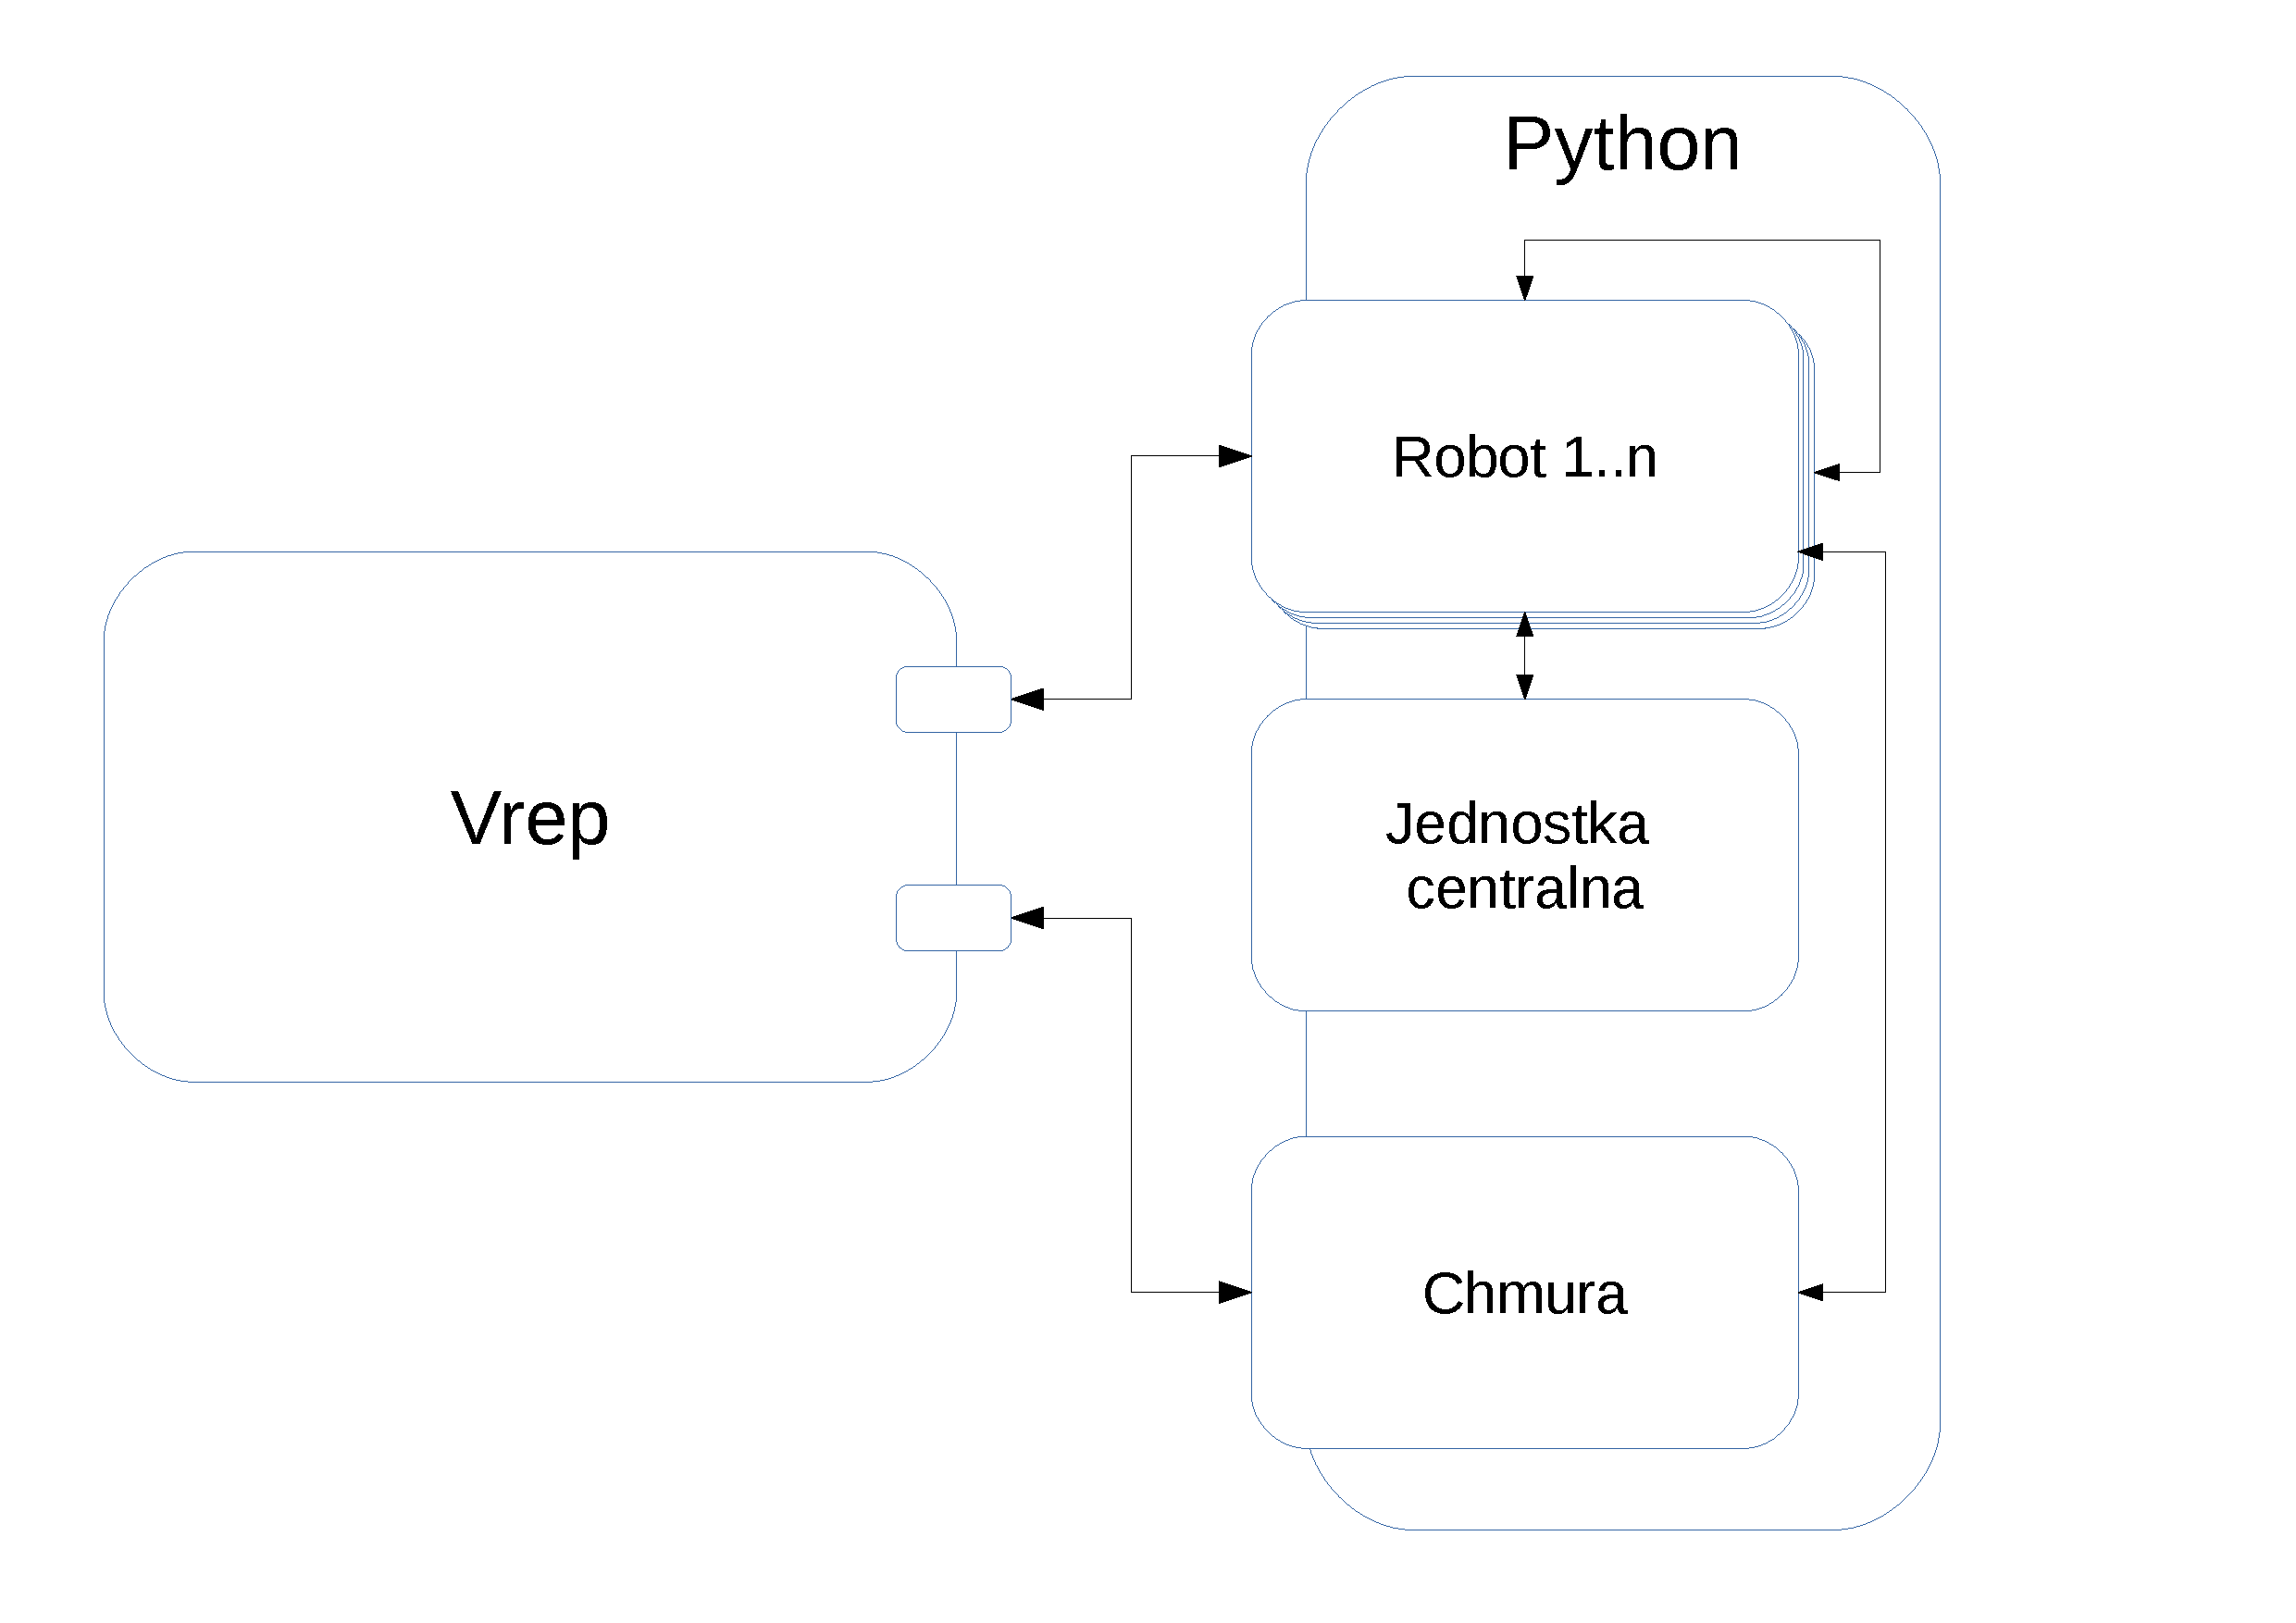
\includegraphics[width=0.9\columnwidth]{img/schemat_sst_1.pdf}
	\caption{Schemat działania systemu.}
	\end{figure}
	Dla robotów, jednostki centralnej oraz chmury stworzone zostaną procesy, które będą się komunikować z symulatorem V-rep:
	\begin{itemize}
		\item procesy robotów będą wysyłać sterowania i odbierać odczyty z czujników przeszkód z symulatora V-rep (V-rep będzie symulować rzeczywiste roboty i rzeczywiste środowisko);
		\item możliwa będzie komunikacja pomiędzy robotami;
		\item jednostka centralna będzie odbierać od robotów odczyty skażenia;
		\item stworzony zostanie osobny proces, który będzie symulował chmurę skażenia; proces ten symulował będzie wartości odczytów czujników skażenia i przekazywał informacje o kształcie i położeniu chmury do V-repa.
	\end{itemize}
	
\section{Realizacja}

\subsection{Roboty}
Wykorzystywane w realizacji zadania roboty Pionieer p3dx wyposażone w ultradźwiękowe czujniki odległości - będą one zapewnione przez symulator V-Rep. Posiadają one napęd różnicowy, pozwalający na dużą swobodę poruszania się po symulowanej przestrzeni. Są przystosowane do rozbudowy o dodatkowe urządzenia -- dzięki czemu mogły by być łatwo dostosowane do realizacji zadania lokalizacji chmury.
Dodatkowo, czujniki stężenia toksycznych substancji będą realizowane w skryptach Pythona, ułatwiając jej symulację. Informacje o jej położeniu i kształcie będą przekazywane do Vrepa, gdzie nastąpi ich wizualizacja.
\subsection{Algorytmy}

\subsubsection{Algorytm poszukiwania chmury}
	Roboty rozpoczynają pracę od ustawienia się w formacji linii -- maksymalna odległość między robotami jest określona wzorem:
	\begin{math}
	d_{max} = 0.7*min(max(z_1,2*z_2))
	\end{math}
	Gdzie:\\
	$d_{max}$ -- maksymalna odległość między robotami\\
	$z_1$ -- zasięg urządzeń komunikacyjnych robotów\\
	$z_2$ -- zasięg czujników odległości\\
	Roboty w ten sposób zaczynają poruszać się do przodu do momentu dotarcia do przeszkody, toksycznej chmury lub granicy obszaru poszukiwań. W przypadku powyższych wydarzeń, uruchamiane są odpowiednie algorytmy.
	Gdy roboty dotrą do końca obszaru poszukiwań, zatrzymują się, przesuwają w bok i kontynuują poszukiwania w drugą stronę, granicząc z poprzednim obszarem poszukiwań.
\subsubsection{Algorytm bug 2}
	Algorytm ten będzie stosowany w przypadku napotkania przeszkody przez robota. Polega on na podążaniu wzdłuż ściany przeszkody do momentu osiągnięcia punktu leżącego za napotkaną ścianą, na przedłużeniu początkowej ścieżki ruchu. Jego działanie zostało przedstawione na rysunku \ref{bug2_img}.
	\begin{figure}[h!]
	\centering
	\includegraphics*[width=0.7\columnwidth]{img/40-0.png}
	\caption{Działanie algorytmu bug 2}
	\label{bug2_img}
	\end{figure}
	W zastosowaniu dla grupy robotów zmodyfikujemy ten algorytm w następujący sposób:
	Gdy robot/roboty wykryją przeszkodę, oceniane jest jej położenie względem środka szeregu. Większość szeregu powinna poruszać się dalej, natomiast pozostałe roboty powinny zacząć omijać przeszkodę w kierunku większości za pomocą algorytmu bug 2, nie przerywając połączenia z siecią. Jego działanie zaprezentowano na rysunku \ref{omijanie}.
	\begin{figure}[H!]
		\includegraphics*[width=0.5\columnwidth]{img/przeszkoda/1.png}
		\includegraphics*[width=0.5\columnwidth]{img/przeszkoda/2.png}
		\includegraphics*[width=0.5\columnwidth]{img/przeszkoda/3.png}
		\includegraphics*[width=0.5\columnwidth]{img/przeszkoda/4.png}
		\caption{Działanie algorytmu bug 2 dla wielu robotów}
		\label{omijanie}
	\end{figure}
	\subsubsection{Algorytm otaczania chmury}
	W momencie napotkania chmury przez któregokolwiek robota, zatrzymuje się on (po osiągnięciu natężenia toksyn określonego programowo). Pozostałe roboty jadą dalej, po łuku -- tak, aby nie przerwać połączenia z siecią. Gdy napotkają określone stężenie chmury, zatrzymują się. Gdy wszystkie roboty zatrzymały się, zwracają się w jedną stronę i zaczynają okrążać chmurę, utrzymując się na granicy stężenia oraz zachowując spójność sieci. Jego działanie przedstawiono na rysunku \ref{otaczanie}.
		\begin{figure}[H!]
			\includegraphics*[width=0.5\columnwidth]{img/chmura/1.png}
			\includegraphics*[width=0.5\columnwidth]{img/chmura/2.png}
			\includegraphics*[width=0.5\columnwidth]{img/chmura/3.png}
			\includegraphics*[width=0.5\columnwidth]{img/chmura/4.png}
			\caption{Działanie algorytmu otaczania chmury}
			\label{otaczanie}
		\end{figure}
\end{document}


